\chapter{Additional \rmfamily{\LaTeX} \sffamily{Formatting}}
\label{ch:ch2}

In this chapter, we'll provide some additional guidelines and useful \LaTeX{} commands for formatting your document.


%{\color{mediumgray} \blindtext}
\section{More {\rmfamily\LaTeX{}} Usage Examples}
In Figure~\ref{fig:brach2} below, we show some pretty blue and grey lines. This is the first figure in \cref{ch:ch2} and you can see that it is numbered accordingly. Notice that the \verb|\ref| command automatically provides the correct numbering for the item being referenced. If you use the \verb|\cref| command, the label (e.g., Figure, Chapter) will be added automatically. For figures and equations, however, \verb|\cref| will abbreviate the labels (i.e., Fig. and Eq.). Either \verb|\ref|, with label provided by you, or \verb|\cref|, with automatic labeling, can be used. 

\begin{figure}[htbp]
	\centering
	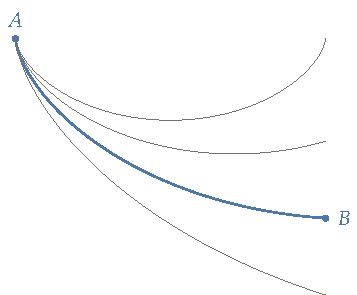
\includegraphics[width=2.2in]{figures/brachistochrone}
	\caption[Short caption to appear in list of figures.]{This is another figure. Some authors have paragraph-like descriptions of their figures that they put into the caption. This is acceptable, but readers don't really want or need a super long caption showing up in their list of figures. The {\ttfamily caption} command provides a nice solution.}
	\label{fig:brach2}
\end{figure}

\section{Bibliography}
Another great feature of \LaTeX{} is that it allows you to create a list or database of books, papers, and other documents that you can easily cite in your document. In engineering, it is common to give your bibliography list the title References and we will follow that convention. \LaTeX{} automatically numbers the citations and builds a bibliography for you.\footnote{The building of your bibliography is actually done by the {\ttfamily biblatex} package. If you use an IDE to work with \LaTeX, this may not be obvious to you.} The bibliography is typeset according the style you specify. The fancy format option of the {\ttfamily byuthesis.cls} class uses the {\ttfamily byubib} bibliography and citation style that produces a numbered list in order of citation. For this document, the file {\ttfamily references.bib} contains the bibliographic reference information that's available for citation in the thesis document. Each reference is created using a defined document type (e.g., {\ttfamily book} or {\ttfamily article}) and is given a cite key (a label) that is used to cite the reference. For example, here is a reference to a book~\scite{book1} and a reference to a doctoral dissertation~\scite{doctoral1}. Journal articles~\scite{journal1} are treated differently than conference papers~\scite{conference1} since their references require slightly different information. Here is a reference to multiple sources at once~\scite{journal2,journal3,journal4}. As another example, here is a reference to a technical report~\scite{techreport1} created using the {\ttfamily @techreport} document type.  Websites can be cited as well~\scite{website1} using the {\ttfamily @online} or {\ttfamily @electronic} document types. The fancy format produces a brief citation in the side margin where the reference is cited and a more detailed citation in the References section at the end of the document.

For each reference entry in your {\ttfamily .bib} file, different information fields will have to be populated. Examples of these fields include, {\em author}, {\em title}, {\em year}, and so on. Different types of publications will have different required fields for you to fill out. There are other types of citations that you may use, such as book chapters and websites. You can manually edit your {\ttfamily .bib} file with a text editor, or you can use one of the several popular apps that are available for editing and organizing your bibliography information (e.g., BibDesk, JabRef).

Digital object identifiers (DOI) enable some nice features within {\rmfamily\LaTeX{}}. Notice that the {\em doi} field for the {\ttfamily journal1} reference in the {\ttfamily references.bib} file includes the DOI {\ttfamily 10.1109/TAP.2004}. This DOI is automatically included as part of the reference in the References list at the end of the document. The DOI in the reference is an active hypertext link to the source document. (Go ahead and click on the DOI in the {\ttfamily template.pdf} document and see what happens.) For citations with a DOI, the title of the citation in the side margin is also an active link to the source document. For all of the side-margin citations, clicking on the citation number will take you to the full reference in the Reference section. From the Reference section, clicking on the citation page number in the side margin will take you back to the location in the document where the reference was originally cited. These features are really great when reading the PDF form of the thesis electronically.

\section{Use of Units}
Units should be appropriately used for all measurements and data presented in the document. Standard abbreviations for units (e.g., m for meters, N for newtons, in. for inches) should be used whenever data is presented. For example, the shaft was 1.23 cm in diameter. Notice that there is a space between the number and the unit, and the unit is typeset in vertical (roman) text and is {\em not italicized}. Italics is reserved for emphasis and for mathematical variables. Periods are not used after abbreviations except in the special case of the abbreviation for inches as in. to avoid confusion with the word in. Units are typically spelled out when they are used without data. For example, newtons are a measure of force, while kilograms are a measure of mass.

\section{Capitalization of Reference Labels}
Throughout your document, you will refer to figures, tables, equations, chapters, appendices, and sections by name (e.g., Figure 2.1, Section 3.4, Equation 2.1, and so on). You may choose to capitalize these reference labels, or to leave them uncapitalized (e.g., figure 2.1, section 3.4, equation 2.1). The choice is yours, just be consistent -- all reference labels should be capitalized, or uncapitalized.

\section{Algorithms}
Software and algorithm development can play an important role in graduate research. Rather than including software code, particularly in the body of the thesis, presenting your algorithms in the form of pseudo-code may be more desirable. The {\ttfamily algorithm} package in \LaTeX{} provides tools for clearly presenting your algorithms. A simple example of the use of this package is presented in Algorithm~\ref{alg:ekf}.

\begin{algorithm}
	\caption{{\color{black} Continuous-discrete extended Kalman filter.}} \label{alg:ekf}
	\begin{algorithmic}[1]
	    \State Initialize:  $\hat{x} = 0$.
	    \State Pick an output sample rate $T_{\textit{out}}$ that is much less than
	    the sample rates of the sensors.
	    \State At each sample time $T_{\textit{out}}$:
	    \For{$i=1$ to $N$}
	        \State $\hat{x} = \hat{x} + \left(\frac{T_{\textit{out}}}{N}\right) \left( f(\hat{x}, u)\right)$
	        \State $A = \frac{\partial{f}}{\partial{x}}$
	        \State $P = P + \left(\frac{T_{\textit{out}}}{N}\right)
	        \left(AP+PA^T + GQG^T\right)$
	    \EndFor
	    \If{a measurement has been received from sensor $i$}
	        \State $C_i = \frac{\partial{c_i}}{\partial{x}}$
	        \State $L_i = PC_i^T(R_i+C_iPC_i^T)^{-1}$
	        \State $P = (I-L_iC_i)P$
	        \State $\hat{x} = \hat{x} +  L_i\left( y_i - c_i( \hat{x})
	        \right)$.
	    \EndIf
	\end{algorithmic}
\end{algorithm}

\section{Landscape Drawings and Tables}
If you have a figure or table that is best presented in landscape format on a full page, the {\ttfamily rotating} package in \LaTeX{} provides a convenient way to do this. Figure~\ref{fig:landscape_dwg} on the following page shows an example a landscape-format drawing. Here is another reference to the Bringhurst text on typography that is included to show how items cited multiple times show up in the References section~\scite{Bringhurst19}.
\begin{sidewaysfigure}
	\centering
	\vspace{1.7in} % use vspace to properly center figure horizontally on page
	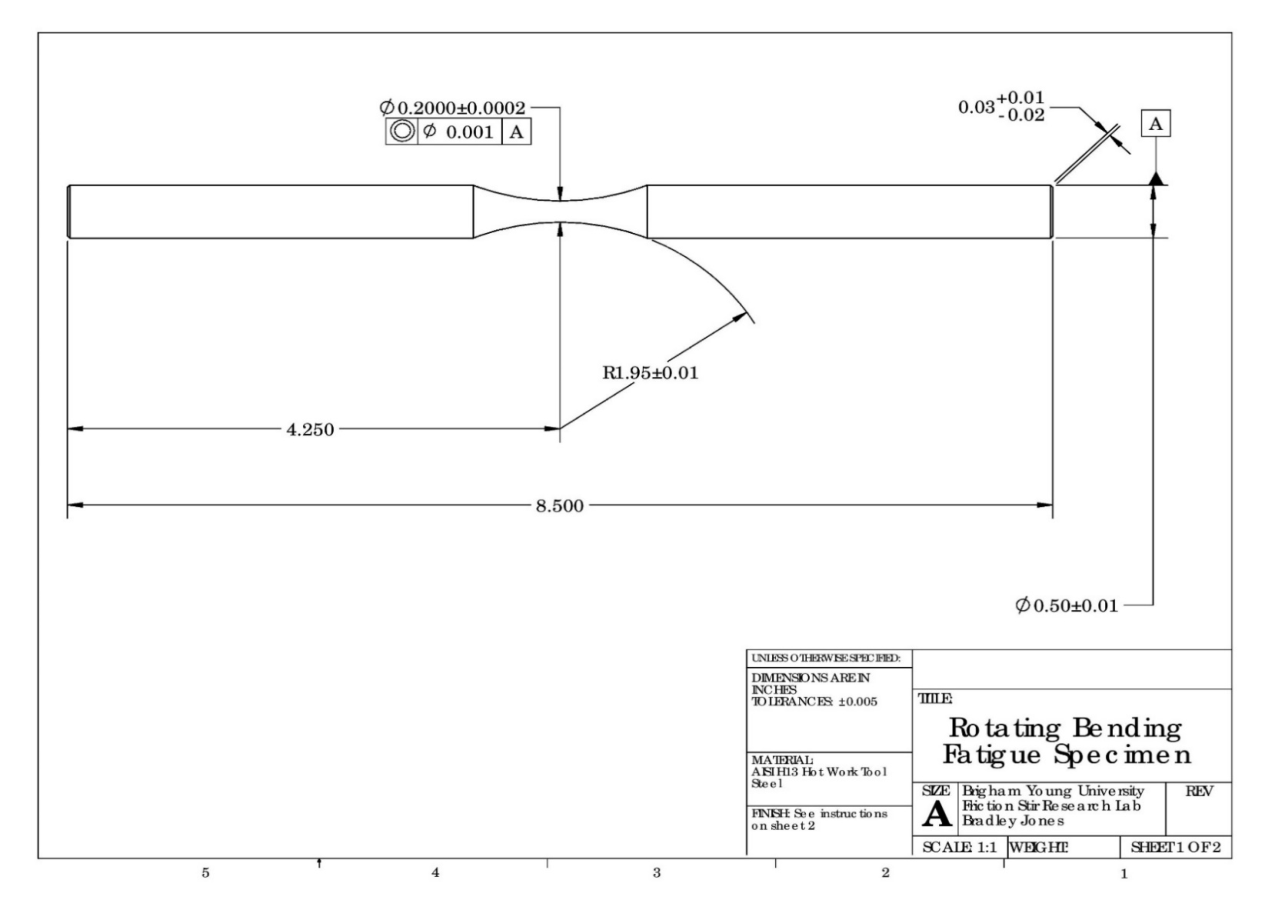
\includegraphics[width=1.0\textwidth]{figures/part_dwg_landscape.pdf}
	\caption{Example of full-page landscape drawing.}
	\label{fig:landscape_dwg}	
\end{sidewaysfigure}


